\section{Optik}

\subsection{Diverses}
\begin{tabular}{p{10cm}p{6cm}}
  %\textbf{Wellenlängen der Spektralfarben} 
  %&
   \textbf{Konstanten} \\
  %\begin{tabular}{|l|l|l|l|}
   % \hline
    %  Wellenlänge in nm & Farbe & Wellenlänge in nm & Farbe \\
     % \hline
      %380 . . . 435 & violett  & 565 . . . 590 & gelb \\
      %435 . . . 465 & blau     & 590 . . . 630 & orange \\
      %465 . . . 485 & blaugrün & 630 . . . 780 & rot \\
      %485 . . . 565 & grün & & \\
      %\hline
  %\end{tabular}
  %&
   \textbf{Vakuumgeschwindigkeit:} \newline 
  $c=299'792'458 \frac{m}{s} \approx 3 \cdot 10^8 \frac{m}{s}$ \\
\end{tabular}

\subsection{Geometrische Optik \kuchling{360} \stoecker{309}}
\renewcommand{\arraystretch}{2}
\begin{tabular}{|p{2.5cm}|p{9.5cm}|p{6cm}|}
  \hline
  \begin{minipage}[]{3.5cm}
    Brechungsgesetz\\
    \kuchling{365} \stoecker{320}\\
  \end{minipage} &
  $\dfrac{\sin \varepsilon_1}{\sin \varepsilon_2} = \dfrac{n_2}{n_1} \qquad n_1
  \sin \varepsilon_1 = n_2 \sin \varepsilon_2 \qquad \varepsilon_1=\varepsilon_1'$ &
  \begin{minipage}[c]{5cm}
    \vspace{0.1cm}
    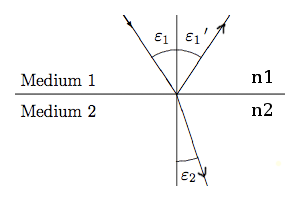
\includegraphics[width=3cm]{./bilder/Brechung.png}
  \end{minipage}\\
  \hline
  \begin{minipage}[]{3.5cm}
    \vspace{0.2cm}
    Brechungsindex\\
    \kuchling{365} \stoecker{320}\\
  \end{minipage}&
  $n=\dfrac{c}{u} \qquad$
  \begin{minipage}[]{4.5cm}
    [c]=Vakumgeschwindigkeit [u]=Lichtgeschwindigkeit
  \end{minipage} &
  \begin{minipage}[]{5cm}
    \renewcommand{\arraystretch}{1}
    \tiny
    \begin{tabular}{ l | l | l | l }
      & & & \\
      Medium & n & Medium & n \\
      \hline
      & & & \\
  		Luft   & 1,000292 & Kronglas (K13) & 1,522 \\
  		Wasser & 1,333    & Flintglas (K2) & 1,620 \\
      &          & Diamant        & 2,417 \\
    \end{tabular}
    \renewcommand{\arraystretch}{2}
  \end{minipage}\\
  \hline
  \begin{minipage}[]{3.5cm}
    Totalreflexion\\
    \kuchling{366} \stoecker{322}\\
  \end{minipage} &
  \parbox{2.5cm}{Für $n_1 > n_2$\\ \\
  $\varepsilon = \arcsin \dfrac{n_2}{n_1} \quad$}
  \begin{minipage}[]{6cm}
    $\varepsilon=\varepsilon_g \Rightarrow$ Grenzfall (ausgezogene Linie)
    $\varepsilon<\varepsilon_g \Rightarrow$ Brechung (gepunktete Linie)
    $\varepsilon>\varepsilon_g \Rightarrow$ Reflexion (gestrichelte Linie)     	
  \end{minipage} &
  \begin{minipage}[c][2.3cm]{4cm}
    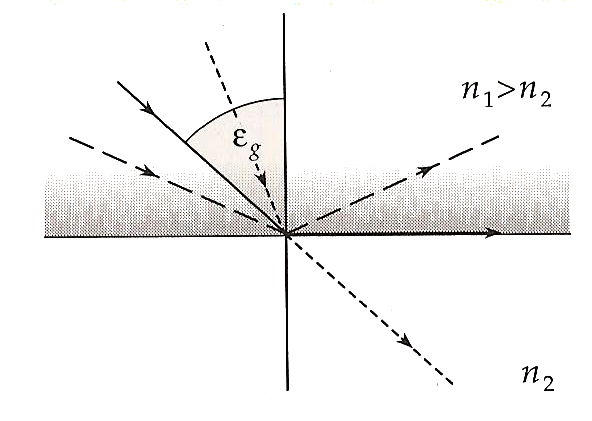
\includegraphics[height=2.2cm]{./bilder/Totalreflexion.png}
  \end{minipage}\\
  \hline
  \begin{minipage}[]{3.5cm}
    \vspace{0.2cm}
    Brennweite\\
    \kuchling{362} \stoecker{316}\\
  \end{minipage} &
  \begin{minipage}[]{6cm}
    Spiegel:\\
    $f=\dfrac{r}{2} \quad$ (für kleine $h$ gilt
    $a = b \approx \dfrac{r}{2}$) \\
    Linse:\\
    $\rightarrow$ Linsenschleifergleichung\\
  \end{minipage} &
  \begin{minipage}[]{6cm}
    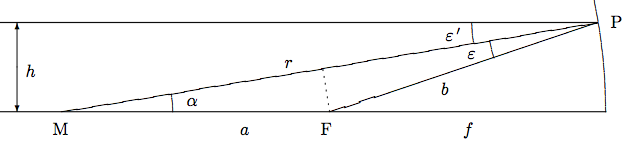
\includegraphics[width=6cm]{./bilder/BrennweiteSphaerischerSpiegel.png}
  \end{minipage}\\
  \hline
  \begin{minipage}[]{3.5cm}
      \vspace{0.2cm}
      Brechkraft,\\
      Linsenschleifer-gleichung\\
  		\kuchling{370}\\
    \end{minipage} & 
    \begin{minipage}{9.5cm}
    $D=\dfrac{1}{f}=\left(\dfrac{n_2}{n_1}-1\right)\left(\dfrac{1}{r_1}+
    \dfrac{1}{r_2}\right) \qquad \underbrace{D_{tot} = D_1 + D_2}_{\text{Abstand von Linsen}\ll f} $ \\
    \parbox{2.6cm}{$\frac{1}{r_1} ; \frac{1}{r_2} = 0$: Plan }
    \parbox{4cm}{
    $r_1, r_2>0$: Konvex\\
    $r_1, r_2<0$: Konkav\\
    }
    \end{minipage}
    &
  	\begin{minipage}[]{6cm}
  		D = Dioptrien [dpt] \quad $1dpt=1m^{-1}$ \\
  		$n_1$ = B.index d. umgebenden Mediums \\
  		$n_2$ = B.index der Linse  
  	\end{minipage} \\
  	\hline
  	Brillengleichung & $D_B = D'_{min} - D_{min} = 
  	\frac{1}{g'_{min}} -\frac{1}{g_{min}}$ 
  	& 
  	\begin{minipage}[]{6cm}
  	\vspace{0.1cm}
  	 $D_B$: Dioptrien der Brille \\
  	 $g'_{min}$:neue Entfernung zum Scharf sehen\\
  	 $g_{min}$: alte Entfernung zum Scharf sehen \\
  	 \vspace{0.1cm}
  	\end{minipage} \\
  	\hline
  \begin{minipage}[]{3.5cm}
    \vspace{2.7cm}
    Abbildungs-gleichungen\\
    \kuchling{363} \stoecker{373}\\
  \end{minipage} &
  \begin{minipage}[c]{3cm}
    $\boxed{\dfrac{1}{f}=\dfrac{1}{g}+\dfrac{1}{b} \quad}$\\ \\
    $\boxed{\dfrac{B}{G}=\dfrac{b}{g}=\alpha}$ \\ \\
    $\boxed{\alpha_{tot} = \alpha_1 \cdot \alpha_2}$   
  \end{minipage}
  \begin{minipage}[c]{5cm}
    \vspace{0.2cm}
    G = Gegenstandshöhe\\
    g = Gegenstandsweite\\
    B = Bildhöhe\\
    b = Bildweite\\
    F = Brennpunkt\\
    f = Brennweite\\
    $\alpha$ = Vergösserungsfaktor \\
    $\alpha < 1$ = verkl., $\alpha > 1$ = vergr.\\
  \end{minipage}
  \begin{minipage}[]{9.5cm}
    \underline{Vorzeichenkonventionen}\\
    -Spiegel konkav / Linse konvex (sammelnd) $\quad \Rightarrow \quad f>0$\\
    -Spiegel konvex / Linse konkav (zerstreuend)$\quad \Rightarrow \quad f<0$\\
    -Bild virtuell $\quad \Rightarrow \quad b<0 \quad\& \quad  B<0$\\
    -Gegenstand virtuell $\quad \Rightarrow \quad g<0 \quad \& \quad G<0$\\
  \end{minipage}&
  \begin{minipage}[]{6cm}
    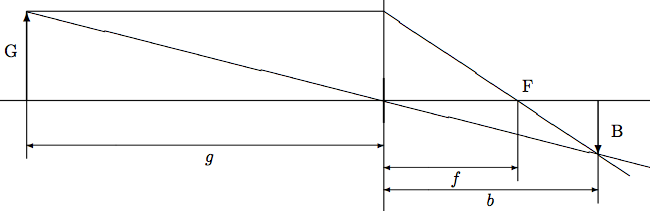
\includegraphics[width=6cm]{./bilder/Abbildungsgleichungen.png}
  \end{minipage}
  
  \begin{minipage}{6cm}
  	\vspace{1cm}
  	Bei reelem Gegenstand:\\
  	-$B > 0$: invertiertes Bild\\
  	-$B < 0$: aufrecht, seitenrichtig
  \end{minipage}\\
  \hline
 \end{tabular}

\renewcommand{\arraystretch}{1}
\newpage

\subsection{Spiegel \kuchling{362} \stoecker{315}}
\begin{minipage}[]{4cm}
  Sammel-/Konkavspiegel\\
  (Hohlspiegel)\\
  $f>0, g>0$
\end{minipage}
\begin{minipage}[]{6.5cm}
  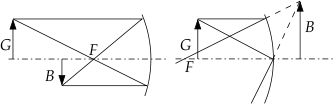
\includegraphics[width=6cm]{./bilder/Konkavspiegel.png}
\end{minipage}
\begin{minipage}[]{8cm}
  \small
  Gegenstand ausserhalb der Brennweite \\
  $\Rightarrow$ reelles, verkleinertes \& verkehrtes Bild $(b>0)$\\ \\
  Gegenstand innerhalb der Brennweite \\
  $\Rightarrow$ virtuelles, vergrössertes \& aufrechtes Bild $(b<0)$
\end{minipage}

\begin{minipage}[]{3.5cm}
  Streu-/Konvexspiegel\\
  (Wölbspiegel)
  $f<0, g>0$
\end{minipage}
\begin{minipage}[]{7cm}
  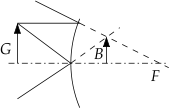
\includegraphics[width=3cm]{./bilder/Konvexspiegel.png}
\end{minipage}
\begin{minipage}[]{8cm}
  \small
  Gegenstand hat stets virtuelles, verkleinertes \& aufrechtes Bild $(b<0)$
\end{minipage}

\begin{minipage}[]{3.5cm}
  Planspiegel
\end{minipage}
\begin{minipage}[]{7cm}
  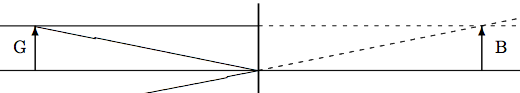
\includegraphics[height=1cm]{./bilder/Planspiegel.png}
\end{minipage}
\begin{minipage}[]{8cm}
  \small
  Bild ist virtuell und gleich gross wie Gegenstand, Bildweite ist gleich
  Gegenstandsweite. Brennpunkt liegt im Unendlichen. $(b<0)$
\end{minipage}

\subsection{Linsen \kuchling{369} \stoecker{331}}
\begin{minipage}[]{3.5cm}
  Sammel-/Konvexlinsen\\
  $f>0,g>0$
\end{minipage}
\begin{minipage}[]{2cm}
  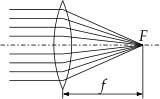
\includegraphics[width=2cm]{./bilder/sammelprinzip.png}
\end{minipage}
\begin{minipage}[]{5cm}
  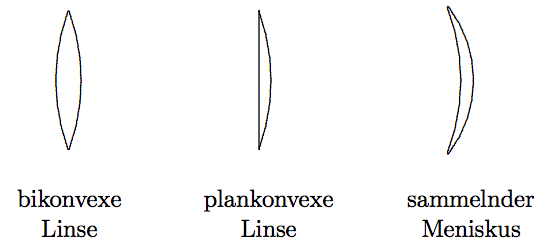
\includegraphics[width=5cm]{./bilder/sammellinsen.png}
\end{minipage}
\begin{minipage}[]{7.5cm}
  \small
  Gegenstand ausserhalb der Brennweite \\
  $\Rightarrow$ reelles, verkleinertes \& verkehrtes Bild $(b>0)$\\ \\
  Gegenstand innerhalb der Brennweite \\
  $\quad \Rightarrow$ virtuelles, vergrössertes \& aufrechtes Bild $(b<0)$
\end{minipage}

\begin{minipage}[]{3.5cm}
  Konkav-/Zerstreuungslinsen\\
  $f<0,g>0$
\end{minipage}
\begin{minipage}[]{2cm}
  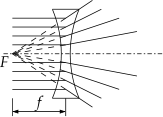
\includegraphics[width=2cm]{./bilder/streuprinzip.png}
\end{minipage}
\begin{minipage}[]{5cm}
  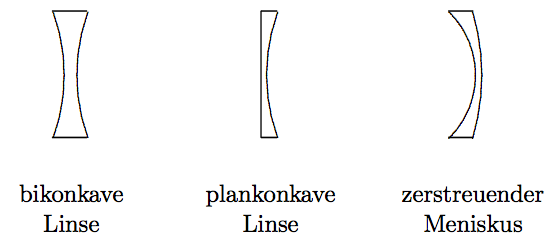
\includegraphics[width=5cm]{./bilder/streulinsen.png}
\end{minipage}
\begin{minipage}[]{7.5cm}
  \small
  Gegenstand hat stets virtuelles, aufrechtes \& verkleinertes Bild $(b<0)$
\end{minipage}

\subsection{Abbildungsfehler}
\begin{tabular}{ll}
  Sph"arische Abberation & Brennweite ist Funktion des Abstands zur optischen
  Achse \\
  Koma & beim schiefen Einfall ($\rightarrow$ Schweiff"ormiger Fehler) \\
  Astigmatismus, Bildfeldw"olbung & vertikal und horizontal $\rightarrow$ andere
  Brennweite (Auge) \\
  Verzeichnung & tonnen- oder kissenf"ormige Verzeichnung eines Quadrates
  ($\rightarrow$ Photogrammetrie) \\
  Chromatische Abberation & wegen Dispersion $\Rightarrow$ Brennweite ist
  Funktion von $\lambda$ (Farbe) \\
\end{tabular}

\subsection{Optische Systeme}
\subsubsection{Kamera \kuchling{378} \stoecker{343}}
\begin{tabular}{lll}
  \parbox{3cm}{
    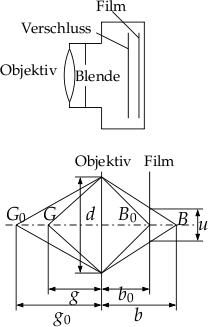
\includegraphics[width=3cm]{./bilder/kamera.png}} &
  \parbox{7cm}{
    Erzeugt reelles, verkleinertes \& umgekehrtes Bild \\
    \\
    $g \;$ Schärfentiefe\\
    $g_0 \;$ Mittlere Gegenstandsweite\\
    $Z \;$ Blendenzahl \\
    $E \;$ Belichtung \\
    $u \;$ Unschärfekreisdurchmesser \\
    $q \;$ Öffnungsverhältnis (Lichtstärke) \\
    $d \;$ Blenden-Durchmesser \\
    $f \;$ Brennweite (z.B. 35mm-Objektiv)} &
  \parbox{8cm}{
    \fbox{$\dfrac{1}{g_{_{min/max}}}=\dfrac{1}{g_0}\pm\dfrac{u}{q\,f^2}$} \parbox{4cm}{
        $+$ für $g_{_{min}}$\\
        $-$ für $g_{_{max}}$} 
        \\
    $B=\dfrac{f}{g-f}G$ \qquad bzw. f"ur $g\gg f\quad B=\dfrac{f}{g}G$\\
    $Z = \dfrac{f}{d} = \dfrac1q$ \qquad $q = \dfrac{d}{f} = \dfrac1Z$ 
    \\
    $E\sim q^2\,t$ \\
    Kleine Blende ($Z=16, \,q=1:16$)\\ 
    $\Rightarrow$ grosse Tiefensch"arfe\\
    Grosse Blende ($Z=4,\,q=1:4$) \\ 
    $\Rightarrow$ viel Licht, kleine Tiefensch"arfe} \\
\end{tabular}

\subsubsection{Lupe \kuchling{381} \stoecker{345}}
\begin{tabular}{lll}
  \parbox{7cm}{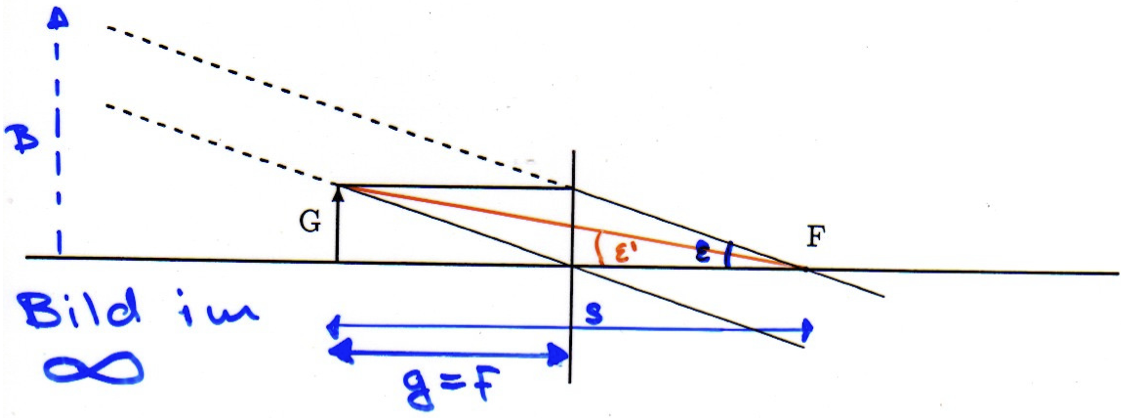
\includegraphics[width=7cm]{./bilder/lupe.png}} &
  \parbox{11cm}{
    Bild ist im Unendlichen, wenn $g=f$\\
    Erzeugt virtuelles, vergrössertes \& aufrechtes Bild \\
    \\
    $V \;$ Vergr"osserung \qquad \qquad $s \;$ deutliche Sehweite (Auge: 25cm)\\
    \qquad $\varepsilon \;$ Sehwinkel mit Lupe \qquad $\varepsilon' = \varepsilon_0 \;$ Sehwinkel
    ohne Lupe = $1/60^\circ$\\
    $V=\dfrac{s}{f}=\dfrac{\tan(\varepsilon)}{\tan(\varepsilon_0)}\Rightarrow\dfrac{s}{g}>
    V_{\text{normal}}$ }
\end{tabular}
\subsubsection{Projektor \kuchling{377}}
\begin{tabular}{ll}
\parbox{6cm}{
  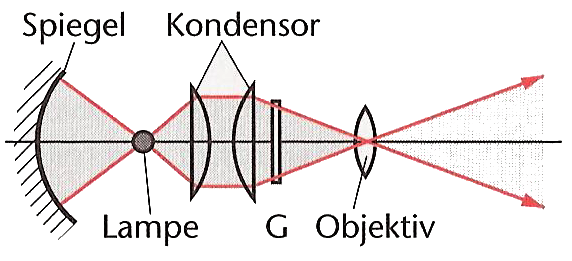
\includegraphics[width=6cm]{./bilder/projektor.png}} &
\parbox{12cm}{
  Erzeugt reelles, vergrössertes \& umgekehrtes Bild \\
  \\
  $\beta \;$ Abbildungsmasstab \\
  $\beta = \dfrac{b}{g} = \dfrac{b}{f}-1$}
\end{tabular}

\subsubsection{Mikroprojektor} 
Erzeugt reelles Bild auf Schirm mit $V=\dfrac{B}{G}=\dfrac{b}{g}$\\

\subsubsection{Mikroskop \kuchling{382} \stoecker{345}}
\begin{tabular}{ll}
  \parbox{8cm}{
    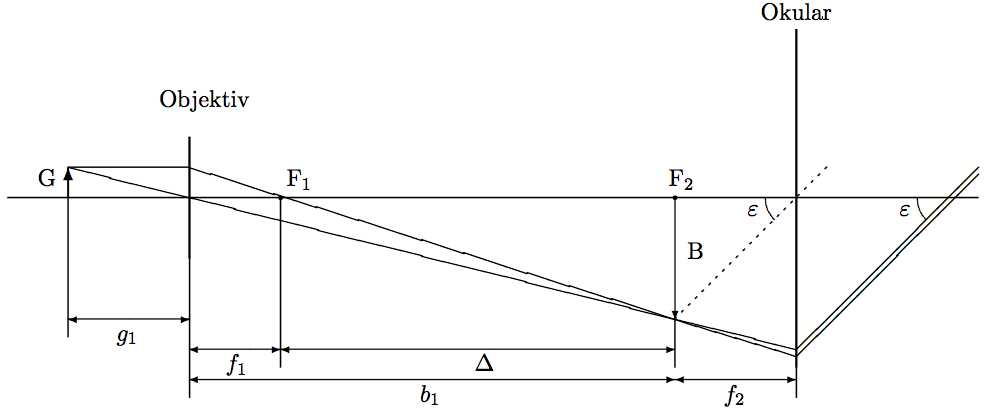
\includegraphics[width=8cm]{./bilder/mikroskop.png}} &
  \parbox{10cm}{
    Erzeugt reelles, vergrössertes \& umgekehrtes Bild. \\
    \\
    $V_1 = \frac{\Delta}{f_1} \;$ Vergrösserung des Objektivs\\
    $V_2 = \frac{s}{f_2} \;$ Vergrösserung des Okulars \\
    \\
    $\Delta = \overline{f_1\,f_2} \;$ Tubuslänge \\
    $V=V_1\,V_2= \dfrac{f_1}{f_2} = \dfrac{\Delta}{f_1} \dfrac{s}{f_2} =
    \dfrac{B}{G} \, \dfrac{s}{f_2}$ }
\end{tabular}

\subsubsection{Keplersches (Astronomisches) Fernrohr \kuchling{383} \stoecker{347}}
\begin{tabular}{ll}
  \parbox{11cm}{
    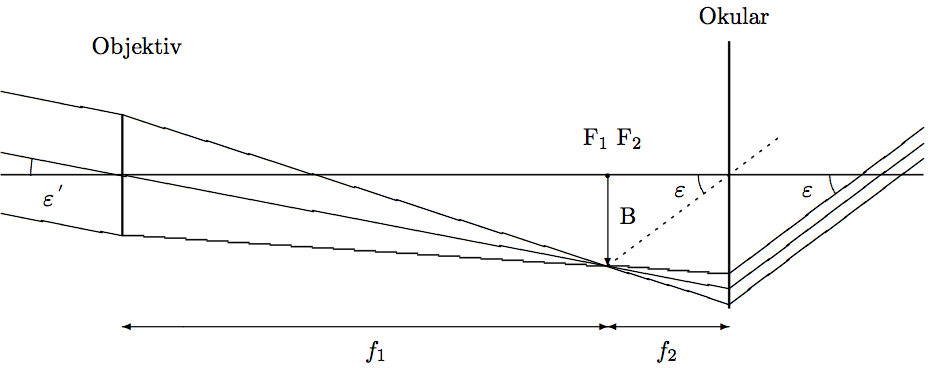
\includegraphics[width=10cm]{./bilder/astron.png}} &
  \parbox{7cm}{
    Erzeugt reelles, vergrössertes \& umgekehrtes Bild. Dies ist ein Spezialfall
    des Mikroskops, wo die \textbf{Gegenstandsweite} auf \textbf{unendlich} ($g \rightarrow \infty$) eingestellt ist. \\
    \\
    $D$ Durchmesser Objektiv \\
    $V$ Vergrösserung\\
    $a$ Abstand Okular-Austrittspupille\\
    $l$ Abstand Objektiv-Okular\\
    $d$ Grösse Austrittspup.\\
    $L$ Lichtstärke }
\end{tabular} \\
$V = \dfrac{\tan(\varepsilon)}{\tan(\varepsilon')} = \dfrac{B/f_2}{B/f_1} =
\dfrac{f_1}{f_2} = \dfrac{D}{d} = \dfrac{f_1+f_2}{a}$ \qquad $l = f_1+f_2$
\qquad $\dfrac{1}{f_1+f_2} + \dfrac{1}{a} = \dfrac{1}{f_2}$ \qquad
$a = \frac{l}{V} $ \qquad $d = \frac{D}{V}$ \qquad $L = d^2 = \left( \frac{D}{V}
\right)^2$

\subsubsection{Diverse \kuchling{384} \stoecker{347}}
\begin{tabular}{ll}
  Terrestr. Fernr. & 
  $V=\left|\dfrac{f_1}{f_2}\right|$ \qquad L"ange: $l=f-|f_2|$ (ent. mit
  Umkehrlinse (ZF), Prismen oder Streul. zur Umkehrung) \\
  Spiegelteleskope &
  Reflexion$\leftrightarrow$Brechung (weniger Lichtv.), k. Dispersion (k. chrom.
  Abberation), Verzug durch Masse  \\
\end{tabular}
\begin{multicols}{2}

\subsection{Konstruktion des Strahlengangs}
\begin{center}
  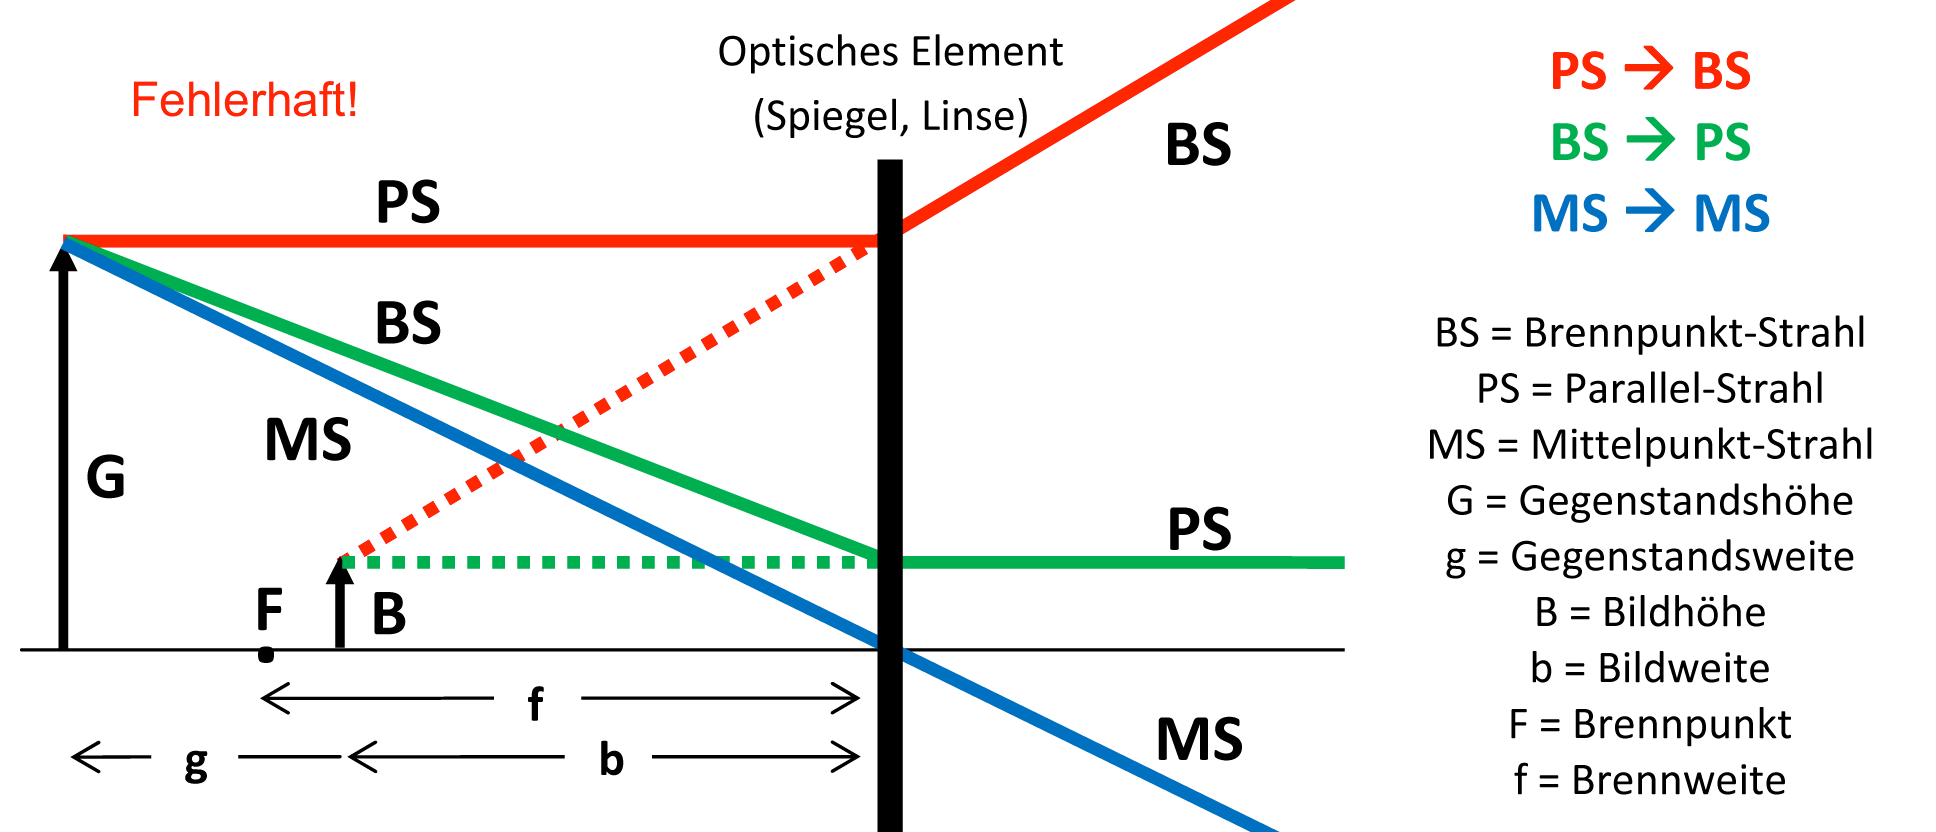
\includegraphics[width=9cm]{./bilder/strahlengang.png}
\end{center}

\subsection{Strichgitter}
$\lambda = g \cdot \frac{\sin(\Phi)}{n}$\\
\\
$\lambda$ = Wellenlänge des Lichts\\
g = Abstand der Striche\\
$\Phi$ = Winkel, bei dem ein Maximum ist\\
n = das wievielte Maximum es ist\\
\end{multicols}